\documentclass[mathserif]{beamer}
\usepackage{beamerthemeshadow}
\usepackage{beamerthemesplit}
%\usetheme{shadow}
\usepackage{graphicx}
\usecolortheme{lily}
%\usepackage{amsmass}
% \usepackage{amssymb,amsfonts,url}

\usepackage{algorithm}
\usepackage{algorithmic}

\usepackage{graphicx}
\graphicspath{{Problems/}}

%\usepackage{CJK}
%\usepackage{pinyin}

%    \begin{figure}
%        \centering
%        \includegraphics[width=0.8\textwidth]{newGeneRep.eps}
%    \end{figure}

% \begin{figure}%
%   \begin{center}%
%     \begin{minipage}{0.70\textwidth}%
%      \includegraphics[width=1.0\textwidth]{comp25000.eps}%
%     \end{minipage}%
%     \begin{minipage}{0.30\textwidth}
%      \includegraphics[width=1.0\textwidth]{comparelabel.eps}%
%     \end{minipage}%
%   \end{center}
% \end{figure}

% \begin{table}
%   {\begin{tabular}{l|rrr}\hline
%       & \multicolumn{3}{c}{Actual number of DCJ operations}\\
%       \# genes &\# genes $\times 1$&\# genes $\times 2$&\# genes  $\times 3$ \\
% \hline
%      (a)~25,000 & 0.5\% ~~&  0.9\% ~~& 1.7\%~~\\
%       (b)~10,000 & 0.8\%~~ &  1.4\% ~~& 2.7\%~~\\
%      (c)~ 1,000 & 2.7\%~~ & 4.7\%~~ & 14.7\%~~\\ \hline
%     \end{tabular}} {}%
% \end{table}

% \begin{eqnarray}
% T(n) &=&  \sum\nolimits_{i=1}^n C_i \\
%      &=&  \# PUSH + \#POP \\
%      &<& 2\times \#PUSH \\
%      &<& 2n \\
% \end{eqnarray}

% \[ 
% \begin{matrix}
% \begin{pmatrix}
% C_{11} & C_{12} \\ 
% C_{21} & C_{22} 
% \end{pmatrix}
% =
% \begin{pmatrix}
% A_{11} & A_{12} \\ 
% A_{21} & A_{22}  
% \end{pmatrix}
% 
% \begin{pmatrix}
% B_{11} & B_{12} \\ 
% B_{21} & B_{22}  
%  
% \end{pmatrix}
%     
%    \end{matrix}
% \]
% 
% 
% \begin{eqnarray}
%  C_{11} &=& (A_{11}\times B_{11}) + (A_{12} \times B_{21}) \\
% C_{12} &=& (A_{11}\times B_{12}) + (A_{12} \times B_{22}) \\
% C_{21} &=& (A_{21}\times B_{11}) + (A_{22} \times B_{21}) \\
% C_{22} &=& (A_{21}\times B_{12}) + (A_{22} \times B_{22}) 
% \end{eqnarray}
% \begin{figure}%
%      \begin{minipage}{0.32\textwidth}%
%       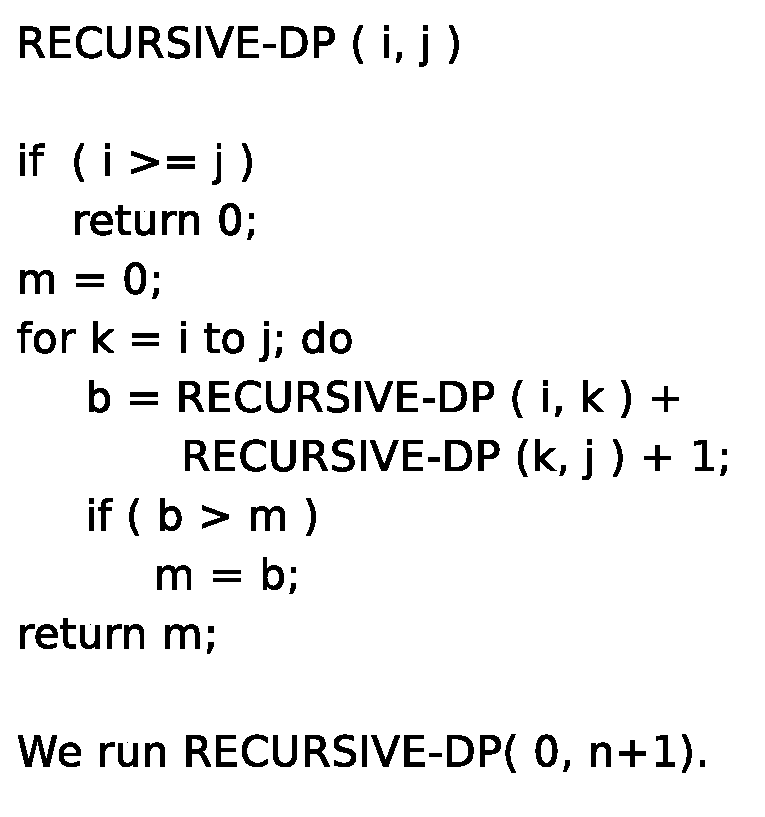
\includegraphics[width=1.0\textwidth]{L7-intervalschedulingdpalgo.eps}%
%      \end{minipage}%
%  \quad
%      \begin{minipage}{0.30\textwidth}
%       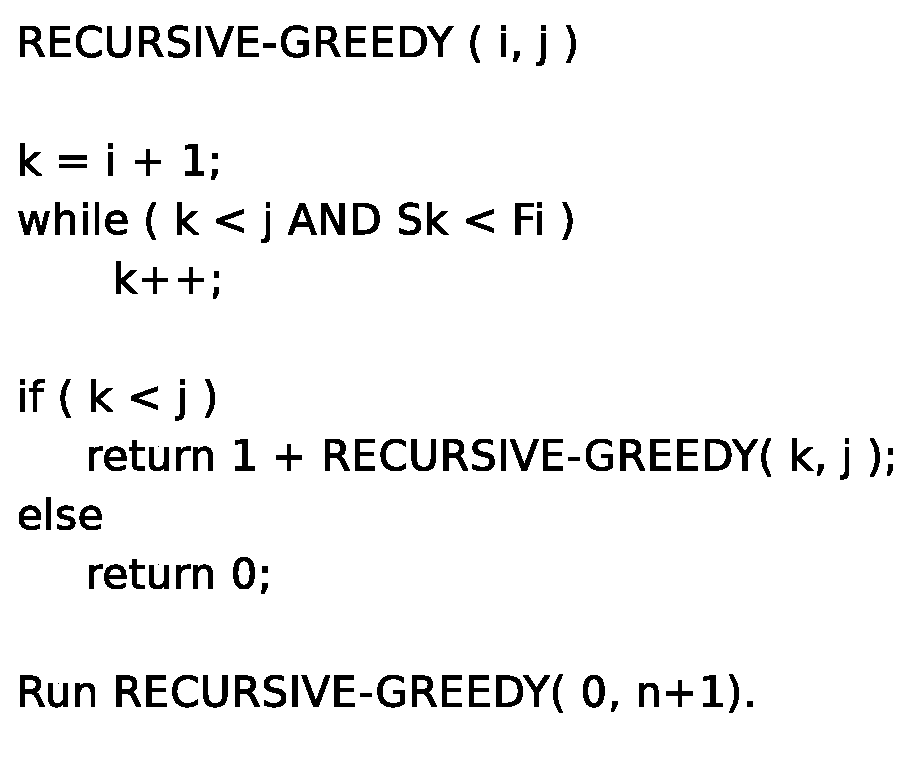
\includegraphics[width=1.0\textwidth]{L7-intervalschedulinggreedyalgo.eps}%
%      \end{minipage}%
%  \quad
%       \begin{minipage}{0.25\textwidth}
%       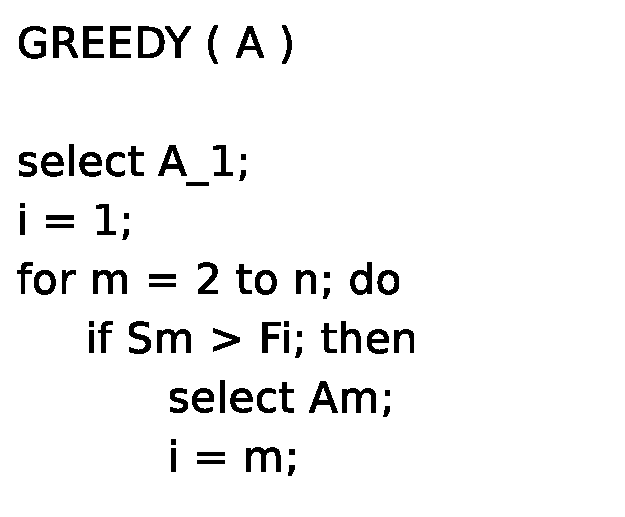
\includegraphics[width=1.0\textwidth]{L7-intervalschedulinggreedyalgo2.eps}%
%      \end{minipage}%
% 
%  \end{figure}

\title{CS612  Algorithm Design and Analysis }
\subtitle{ Lecture 20. {\sc MaxCut} problem: random sampling, derandomization, and semi-definite programming
\footnote{The slides are made based on Approximation Algorithms for NP-Hard problems by D. S. Hochbaum, Computational Complexity by C. H. Papadimitriou, and a report by D. P. Williamson.  } }
 \author{ Dongbo Bu \\
 \ \\
 {\small Institute of Computing Technology \\ 
 Chinese Academy of Sciences, Beijing, China}
}

 
 \date{}

\begin{document}
%\begin{CJK}{UTF8}{cyberbit}
% 
\frame[allowframebreaks]{\titlepage}

\frame[allowframebreaks]{
\frametitle{Outline}
\begin{itemize}
\item Introduction to {\sc MaxCut} problem; 
\item NP-Hardness of {\sc MaxCut} problem;
\item Local search algorithm; 
\item Dumb-randomization algorithm and derandomization; 
\item ``LP+RR'' algorithm by Arora, et al; 
\item Semi-definite programming method;
\end{itemize}
}

\frame{
\frametitle{ {\sc MaxCut} problem }
\begin{block}{}
{\bf INPUT: } An undirected graph $G=<V,E>$.  \\

{\bf OUTPUT: } A cut of $V=A\cup B$, $A\cap B = \phi$, such that the number of edge crossing the cut is maximized. 
 
\end{block}

\begin{figure}
          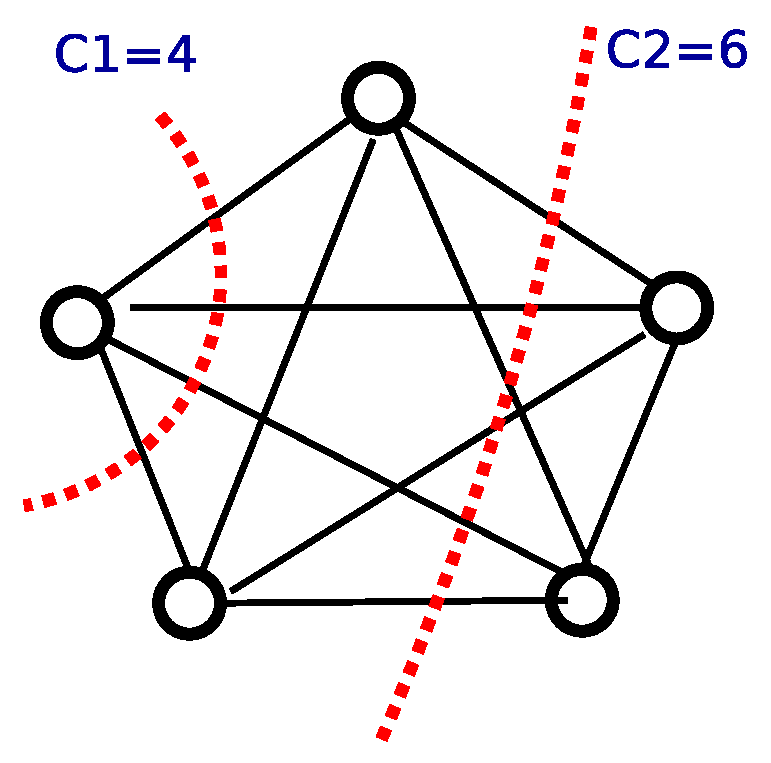
\includegraphics[width=2in]{L20-maxcutexample.eps}
\end{figure}
}    

\frame[allowframebreaks]{
\frametitle{ Hardness of {\sc MaxCut} problem. }
\begin{Theorem}
 {\sc MaxCut} problem is NP-Hard. 
\end{Theorem}
Proof: \\
(Reduction from {\sc NAESAT } to {\sc MaxCut}.) \\
Gaudget: tri-angle. (max cut = 2) 
\begin{itemize}
\item Nodes: $G$ has $2n$ nodes, including $x_i$ and $\neg x_i$ for each variable $i$; 
\item Edges: 
	\begin{enumerate} 
	\item 
	Connecting $x_i$ and $\neg x_i$ with $n_i$ edges, where $n_i$ is the total number of occurence of $x_i$ and $\neg x_i$. 
	\item For each clause $x_i \vee x_j \vee x_k$, draw a tri-angle; for a clause $(x_1 \vee x_2) $, draw two parallel lines $(x_1, x_2)$, $(x_1, x_2)$.
	\end{enumerate}
\end{itemize}

e.g.:  \\
$(x_1 \vee x_2 ) \wedge ( x_1 \vee \neg x_2 \vee \neg x_3 ) \wedge ( \neg x_1 \vee \neg x_2 \vee x_3 )$ $\Leftrightarrow$ \\ 
$(x_1 \vee x_2 \vee x_2 ) \wedge ( x_1 \vee \neg x_2 \vee \neg x_3 ) \wedge ( \neg x_1 \vee \neg x_2 \vee x_3 )$

\begin{figure}
    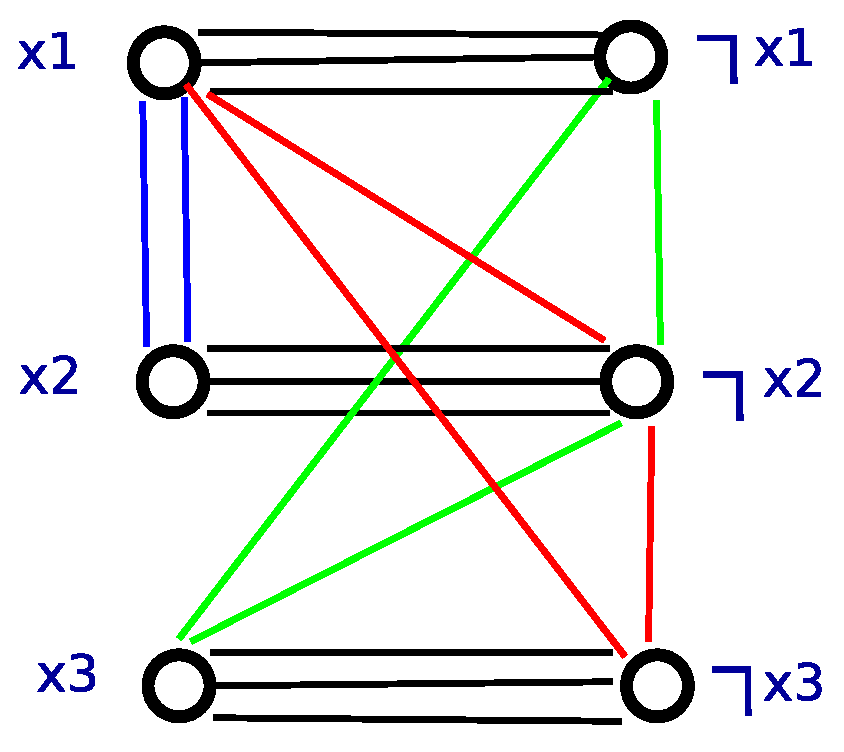
\includegraphics[width=2in]{L20-maxcuteNPhardproof.eps}
\end{figure}

Claim: there is a cut with size $k \ge 5m$ in $G$ iff the NAESAT instance is satisfiable. 

\begin{itemize} 
\item $\Rightarrow:$ \\ 
If $G$ has a cut $S$ of size $5m$ or more, w.l.o.g, we can assume $x_i$ and $\neg x_i$ are in different side, which contributes $3m$ edges to the cut. The other $2m$ edges come from the tri-angles. Constructing an assignment to set all literals in $S$ to be TRUE. All clauses are NAESAT under this assignment. 

$\Leftarrow:$ \\
Let $S$ be the literals that are true. Then the cut $(S, V-S)$ has size $3m+2m=5m$. 

\end{itemize}
}    

\frame{
\frametitle{A local search algo } 

see Lec14.ppt. 
}

\frame
{
\frametitle{ A dumb randomized algorithm } 
{\bf Algorithm}\\
\begin{enumerate} 
 \item $A \leftarrow \phi$, $B \leftarrow \phi$,; 
 \item for i = 1 to n 
 \item 	 \quad if random( $\tfrac{1}{2}$ ) = 1 
 \item   \qquad  $A=A\cup \{i\}$; 
 \item   \quad else
 \item 	 \qquad  $B=B\cup \{i\}$; 
\end{enumerate}
\begin{Theorem} 
 [Sahni, Gonzalez '76] DumbRandom is a $\tfrac{1}{2}$-approximation algorithm.  
\end{Theorem}
}

\frame
{
\begin{Proof} 
 \begin{itemize} 
  \item We define a random variable $x_{ij} = 1 $ iff $i$ and $j$ are not in $A$ simultanously, and $x_{ij}=0$ otherwise. 
  \item We define $W=\sum_{i<j} w_{ij}x_{ij}$. We have: 
   \begin{eqnarray} 
    E(W) & = & E(\sum_{i<j} w_{ij}x_{ij}) \\ 
         & = & \sum_{i<j} w_{ij} E(x_{ij}) \\ 
  & = & \tfrac{1}{2} \sum_{i<j} w_{ij} \\ 
  & \geq  & \tfrac{1}{2} OPT
   \end{eqnarray}
 \end{itemize}

\end{Proof}
}

\frame[allowframebreaks]{
\frametitle{ Derandomization } 
\begin{itemize} 
 \item Changing a randomized algorithm to a deterministic algorithm: Algorithmic derandomization techniques look at a particular randomized algorithm, and using the inherent properties of the problem, analyze the randomized algorithm better to come up with ways to remove randomness from that algorithm. 
 \item Basic idea: conditional expectance. 
e.g. Since
$E( W ) = \tfrac{1}{2} E( W | v_1 \in A  ) + \tfrac{1}{2} E( W | v_1 \in B  )$ 
We have $ E(W) \leq \max \{ E( W | v_1 \in A  ),  E( W | v_1 \in B  ) \} $. 
 \item Derandomization strategy: {\bf put $v_{i+1}$ into $A$  if $E( W | v_1,...,v_i \text{ are determined}, v_{i+1} \in A  ) \geq E( W | v_1,...,v_i \text{ are determined}, v_{i+1} \in B  )$}. 
 \item Repeatedly applying this strategy, we have: 
\begin{eqnarray} 
 \tfrac{1}{2} OPT &\leq& E(W) \\ 
 &\leq& E( W | v_1 \text{ is determined according to the strategy} ) \\ 
 &\leq& E( W | v_1, v_2 \text{ are determined according to the strategy} ) \\ 
 & & ......... \\ 
 & \leq & E( W | v_1, v_2, ..., v_n \text{ are determined according to the strategy} )
\end{eqnarray}


\begin{figure}
          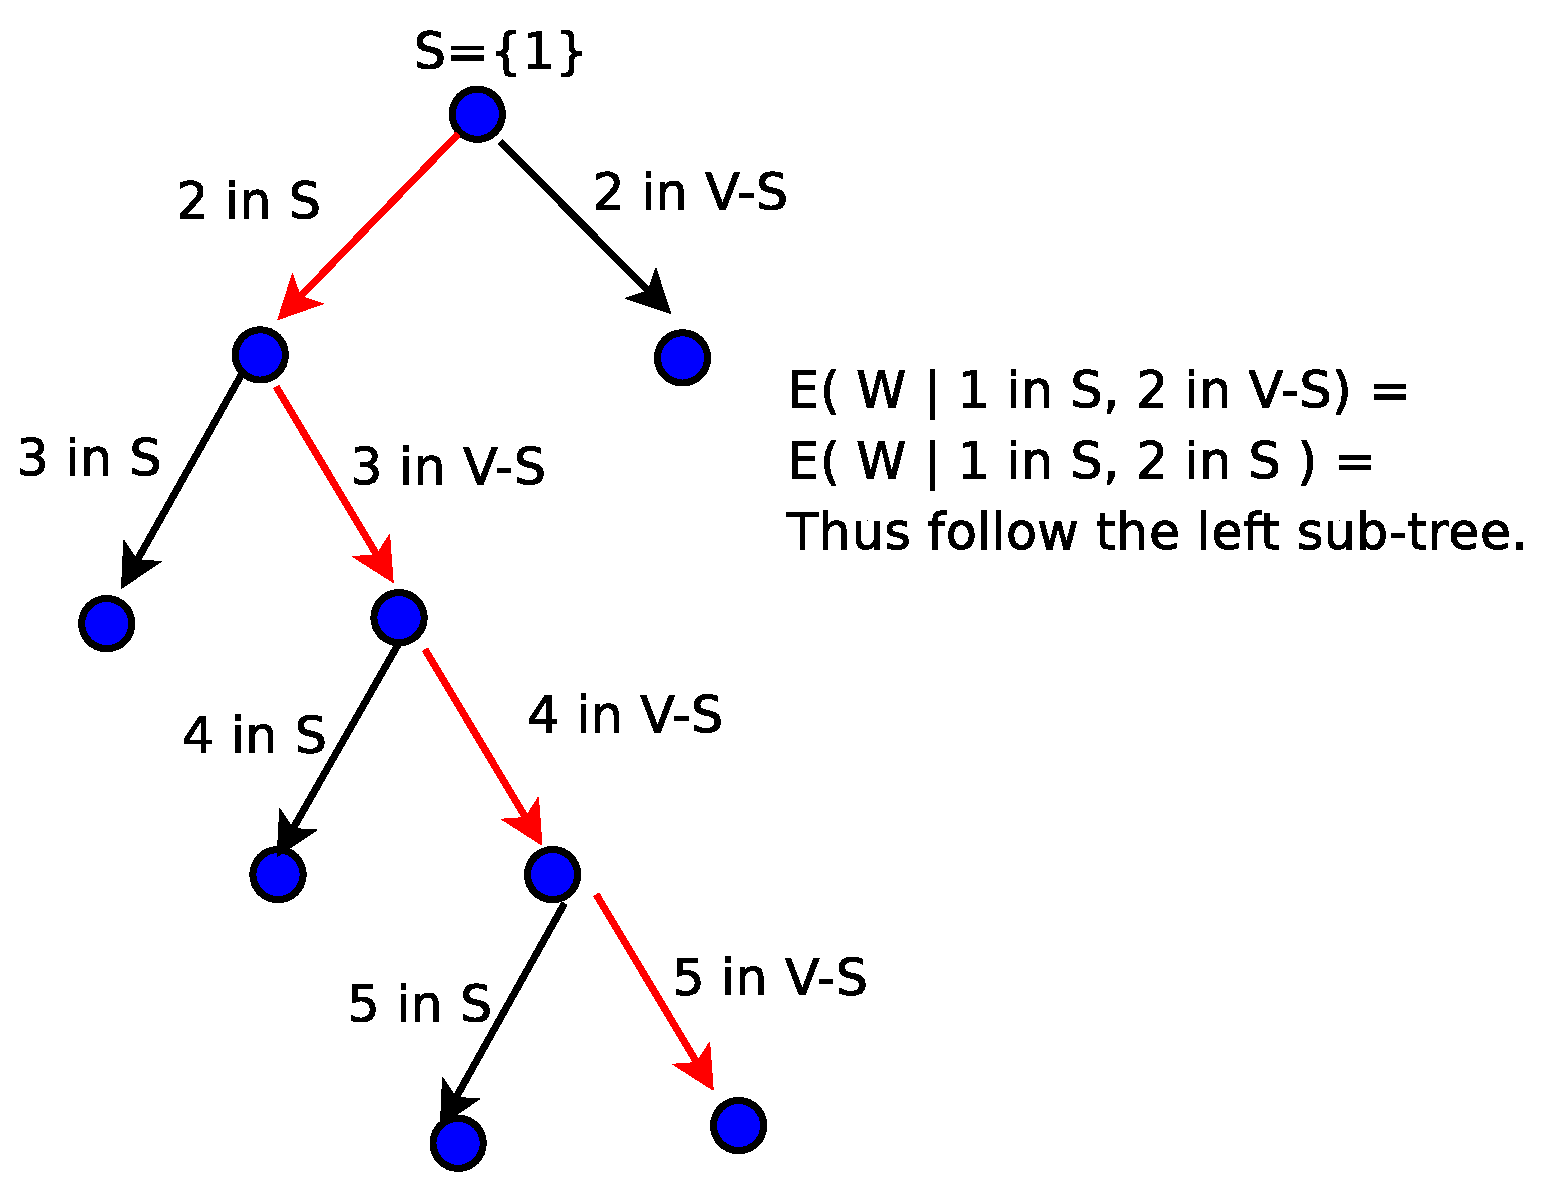
\includegraphics[width=2in]{L20-derandomizationtree.eps}
\end{figure} 

\item Question: how to calculate  $E( W | v_1,...,v_i \text{ are determined}, v_{i+1} \in A  )$? 

\begin{figure}
          \includegraphics[width=2in]{L20-maxcutderandomization.eps}
\end{figure} 


$E( W | v_1,...,v_i \text{ are determined}, v_{i+1} \in A  ) = k + m_B + \tfrac{1}{2} ( m - k - m_A - m_B - l )$ 
$E( W | v_1,...,v_i \text{ are determined}, v_{i+1} \in B  ) = k + m_A + \tfrac{1}{2} ( m - k - m_A - m_B - l )$ 

Thus, the strategy can be rewritten as:\\ 
 \item Derandomization strategy: {\bf put $v_{i+1}$ into $A$  if $m_A \leq m_B$}. 

{\bf Algorithm:}
\begin{enumerate} 
 \item $A \leftarrow \{ v_1\}$, $B \leftarrow \phi$,; 
 \item for i = 2 to n 
 \item   \quad put $i$ into A or B to maximize the cut size; 
\end{enumerate}
 
\end{itemize}

}

% shaomingfu

\frame{
\frametitle{ Chernoff bound } 
\begin{Theorem} 
Let $x_1,x_2,...,x_n$ be $n$ independent $0/1$ random variabless (not necessarily from the same distribution). Let $X=x_1+x_2+...+x_n$, and $\mu = E[ X ] $. For $0\leq \delta \leq 1$, \\
$\Pr [ X \geq (1+\delta) \mu ] \leq e^{ - \tfrac{1}{3} \mu \delta^2 } $ and \\
$\Pr [ X \leq (1-\delta) \mu ] \leq e^{ - \tfrac{1}{2} \mu \delta^2 } $. 
\end{Theorem} 

} 

\frame{
\frametitle{ Hoeffding bound } 

\begin{Theorem} 
Let $x_1,x_2,...,x_n$ be $n$ independent random variabless (not necessarily from the same distribution, and $x_i = 0$ or $\alpha_i$, where $\alpha_i \leq 1$ . Let $X=x_1+x_2+...+x_n$, and $\mu = E[ X ] $. For $0\leq \delta \leq 1$,  \\
$\Pr [ X \geq (1+\delta) \mu ] \leq e^{ - \tfrac{1}{3} \mu \delta^2 } $ and  \\
$\Pr [ X \leq (1-\delta) \mu ] \leq e^{ - \tfrac{1}{2} \mu \delta^2 } $. 
\end{Theorem}
} 

\frame[allowframebreaks]
{
\frametitle{ LP+RR Algorithm for dense graph } 

\begin{itemize}
 \item 
A quadratic programming model: 
\[
\begin{array}{rrrrrrrrl}
 \max & \sum_{i=1}^n x_i \sum_{ (i,j) \in E } (1-x_j)  \\
 s.t. & x_i \in \{0,1\} \\
\end{array} \nonumber
\]


\item Definition: let  $ZN(x,i)$ denote the number of neighboors in $V-S$ of $i$ under solution $x$. 
%\item Suppose $ZN(x,i)$ are known, then the quadratic programming problem is essentially an ILP problem.
\[
\begin{array}{rl}
 \max & \sum_{i=1}^n x_i ZN(x,i) \\
 s.t. & x_i \in \{0,1\} \\
\end{array} \nonumber
\]
\end{itemize}
 
\begin{itemize}
\item Let $x^*$ denote the an optimal solution. 
\item Suppose we have high-quality estimation $Z_i$ of $ZN(x^*,i)$, i.e., $Z_i - \epsilon n \leq ZN(x^*,i) \leq Z_i + \epsilon n $. 
\item 
Then we can approximate the quadratic model through the following LP model: 
\end{itemize}
\[
\begin{array}{rl}
 \max & \sum_{i=1}^n y_i Z_i \\
 s.t. & \sum_{(i,j) \in E } (1-y_j) \leq Z_i + \epsilon n \\
      & \sum_{(i,j) \in E } (1-y_j) \geq Z_i - \epsilon n \\ 
      & y_i \in \{0,1\} \\
\end{array} \nonumber
\]

}

\frame[allowframebreaks]
{
Assumption: the graph is dense, i.e., $|E| = \alpha n^*$ and $w_{ij} = 1$. \\
Observations: 
\begin{enumerate} 
 \item $OPT \geq \tfrac{\alpha}{2} n^2$. (Probability method proof: $E( W ) \geq \tfrac{\alpha}{2} n^2$ $\Rightarrow$ $OPT \geq \tfrac{\alpha}{2} n^2$.)
 \item $x^*$ is also a feasible solution of the LP model. 
 \item The objective function of $x^*$ in the LP model is close to that in the quadratic model, (denoted as $OPT=\sum_i ( ZN(x^*,i)x_i^*$). Therefore, $Z_{LP} \geq (1-\tfrac{2\epsilon}{\alpha}) OPT$. 
\end{enumerate}
\begin{eqnarray} 
 \sum_{i=1}^n Z_i x_i^* & \geq  & \sum_i ( ZN(x^*,i) - \epsilon n ) x_i^*  \\ 
&=& \sum_i ( ZN(x^*,i) x_i^* - \epsilon n  \sum_i  x_i^*  \\
&\geq& OPT - \epsilon n^2  \quad ( \sum_i  x_i^* \leq n ) \\  
&\geq& (1-\tfrac{2\epsilon}{\alpha}) OPT 
\end{eqnarray}

``LP+RR'' method by Arora, Karger, and Karpinski, '95. \\
{\bf Algorithm}\\
\begin{enumerate}
 \item Get $Z_i$ from genie; 
 \item Solve LP, get $y^*$; 
 \item For all node $i$ in $V$, 
 \item \quad if random($y_i^*$) = 1
 \item \qquad $x_i'=1$;  (Add $i$ to $S$)
 \item \quad else 
 \item \qquad $x_i'=0$; (Add $i$ to $V-S$)
\end{enumerate}
} 

\frame[allowframebreaks]{
\frametitle{Analysis}
{\bf Claim:} $\sum_i x_i' ZN(x',i) \geq (1-\tfrac{5\epsilon}{\alpha} ) OPT$ with high probability. \\
{\bf Proof: }

{\bf Fact 1:} With high proability, $ZN(x',i)$ is close to $ZN(y^*,i)$ \\

\begin{eqnarray}
 E( ZN(x',i) ) & = & \sum_{(i,j)\in E} E( 1-x'_j)  \\ 
               & = & \sum_{(i,j)\in E} ( 1 - y_j^* ) \\ 
               & = & ZN(y^*,i)
\end{eqnarray}
Thus with high proability, $ZN(x',i)$ is close to $ZN(y^*,i)$. Speficically, 
\begin{eqnarray}
\Pr [ ZN(x',i) &\leq &( 1 - \delta) ZN(y^*,i) ]\\
 & \leq & e^{ - \tfrac{1}{2} ZN( y^*, i) \delta^2} )   \\
& \leq  & e^{c \ln n } \quad \text{ ( setting } \delta^2=\min\{ 1, \tfrac{2c\ln n }{ ZN(y^*,i) } \} ) \\ 
& = & n^{-c} 
\end{eqnarray}

{\bf Fact 2:} With high proability, $\sum_i x_i' Z_i $  is close to $ \sum_i Z_i y_i^*$. 


Since $E(\sum_i x_i' Z_i ) = \sum_i y_i^* Z_i$, we apply the Hoeffding bound to get 
$\Pr[ \sum_i x_i' \tfrac{Z_i}{Z_{max}}  \leq (1-\delta) \sum_i y^*_i \tfrac{Z_i}{Z_max} ] \leq n^{-c}$ , where $\delta=\min\{1, \tfrac{2c\ln n }{ \sum_i y_i^* \tfrac{Z_i}{Z_{max}} } \}$, $Z_{max} = \max_i\{ Z_i\}$ to ensure $\tfrac{Z_i}{Z_{max}} \leq 1 $. 
Thus with high probability, we have: 
\begin{eqnarray}
 \sum_i x_i' Z_i &\geq&  ( 1-\delta) \sum_i Z_i y_i^* \\ 
&=& ( 1 - \min \{  1, \tfrac{2c\ln n }{ \sum_i y_i^* \tfrac{Z_i}{Z_{max}} } \} ) \sum_i Z_i y_i^*  \\  
& \geq & \sum_i Z_i y_i^* - \sqrt{ 2Z_{max} c \ln n \sum_i y_i^* Z_ i } \\
& \geq & \sum_i Z_i y_i^* - n \sqrt{ 2 c n \ln n }  
\end{eqnarray}

{\bf Fact 3: }
\begin{eqnarray} 
 \sum_i x_i' ZN(x', i) &\geq& \sum_i x_i' (1-\delta) ZN(y^*, i) \\
& \geq & \sum_i x_i' ( ZN(y^*, i) - \sqrt{ 2c \ln n ZN(y^*, i) } )  \\ 
& \geq & \sum_i x_i' ( Z_i - \epsilon n - \sqrt{ 2c \ln n ZN(y^*, i) } ) \\ 
& \geq & \sum_i x_i'  Z_i -  ( \epsilon n + \sqrt{ 2c  n \ln n } ) \sum_i x_i' \\ 
& \geq & \sum_i y_i^*  Z_i - n\sqrt{2cn\ln n } - ( \epsilon n + \sqrt{ 2c  n \ln n } ) \sum_i x_i' \\  
& \geq & \sum_i y_i^* Z_i - 2 n\sqrt{2cn\ln n } -  \epsilon n^2  \\  
& \geq & ( 1 - \tfrac{2\epsilon }{ \alpha } ) OPT - \tfrac{2\epsilon}{\alpha} OPT - o(1) OPT  \\ 
& \geq & ( 1 - \tfrac{5\epsilon }{ \alpha } ) OPT  \\ 
\end{eqnarray}

}

\frame[allowframebreaks]{
\frametitle{How to yield a good approximation $Z_i$? }
\begin{figure}
          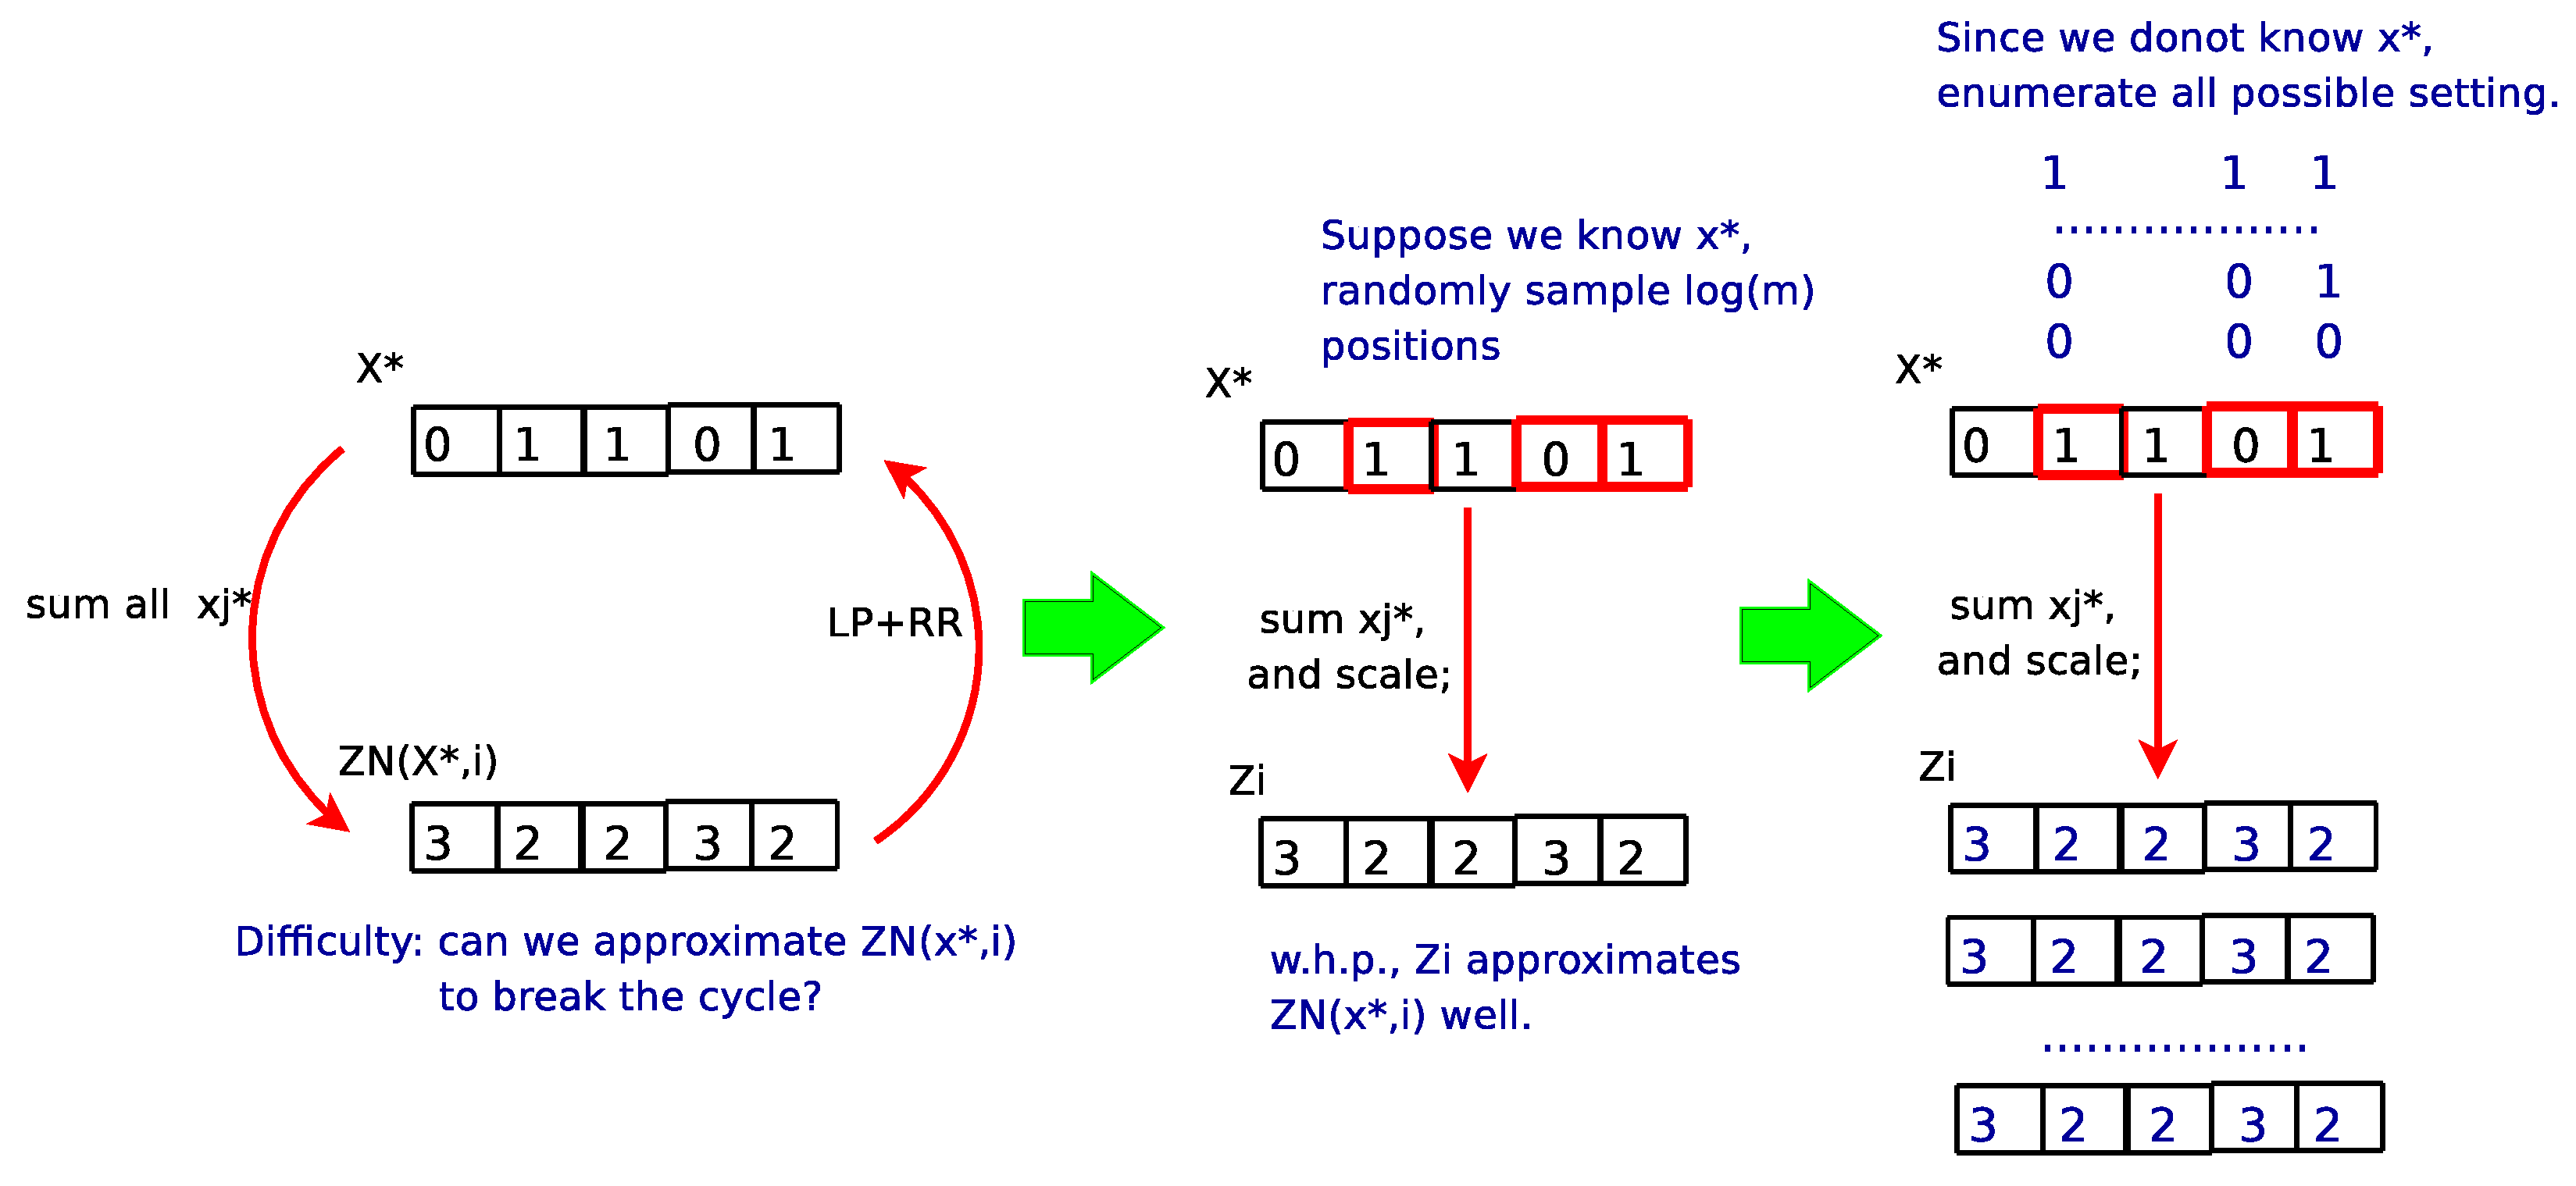
\includegraphics[width=4.6in]{L20-basicidea.eps}
\end{figure} 

\begin{itemize}
 \item Remaining difficulty: how to approximate $ZN(x^*,i)$ by $Z_i$? 
 \item ``Random sampling + enumeration'' again! 
 \begin{enumerate}
  \item Random sampling:   \\ 
   Suppose $x^*$ are known. Pick random subset $S$ of $c\log n / \epsilon^2$ vertices. Set $Z_i = \tfrac{n}{|S|} \sum_{(i,j) \in E, j \in S}  (1-x*_j)$. The with high probability, we have: 
  $ZN( x^*, i) - \epsilon n \leq Z_i \leq ZN( x^*, i) + \epsilon n $. 
  \item Enumerating:  However, $x^*$ are unknown. How to calculate $Z_i$? Enumerating all possible setting of $x_j$ for $j \in S$. This will take poly-time. \\ 
 \end{enumerate}

\end{itemize}
} 
  

\frame[allowframebreaks]{
\frametitle{Semi-definite programming}

A SDP can be formulated as: 

\[
\begin{array}{rrrrrrrrl}
 \max & \sum c_{ij} x_{ij}  \\
 s.t. & \sum a_{ijk} x_{ij} &=& b_k \\ 
      & X=(x_{ij})  \text{ is symmetric and SDP } \\
\end{array} \nonumber
\]

Equivalent to vector programming: 
\[
\begin{array}{rrrrrrrrl}
 \max & \sum c_{ij} ( \vec{ v_i }  \bullet \vec{ v_j } )  \\
 s.t. & \sum a_{ijk} ( \vec{ v_i }  \bullet \vec{ v_j } )  &=& b_k \\ 
      & \vec{ v_i }  \in R^n \\
\end{array} \nonumber
\]

Reason: A PSD matrix $X$ can  be decomposed as $X=V^T V$ for some $V \in R^{m\times n}$. 
Note: SDP (and VP) can be solved in poly-time using the ellipsoid method or the interior-point technique. 
}

\frame[allowframebreaks]{ 
\frametitle{ {\sc MaxCut} using SDP } 

 A quadratic model of {\sc MaxCut}: 
\[
\begin{array}{rrrrrrrrl}
 \max & \tfrac{1}{2} \sum_{i<j} w_{ij} ( 1- y_i y_j) \\ 
 s.t. & y_i \in \{+1,-1\}  \\ 
\end{array} \nonumber
\]

A vector programming relaxation VP: 

\[
\begin{array}{rrrrrrrrl}
 \max & \sum \tfrac{1}{2} w_{ij} ( 1 - \vec{ v_i }  \bullet \vec{ v_j } )  \\
 s.t. & \vec{ v_i }  \bullet \vec{ v_i }   = 1  \\ 
      & \vec{ v_i }  \in R^n \\
\end{array} \nonumber
\]

Note: to see VP is a relaxation of the original quadratic model, we can view $y_i$ as a 1-dimensional vector. Thus, any feasible solution to the quadratical model is also feasible to the VP model. Implication: $Z_{VP} \geq OPT$. 

}

\frame[allowframebreaks]{
\frametitle{ VectorRounding algorithm}
\begin{itemize}
 \item We can solve the vector programming model in poly-time. 
 \item Question: how to convert the solution to VP to a solution to the quadratic model? Vector rounding!
 \begin{enumerate} 
  \item Solve vector programming problem to get vectors $\vec{ v^*}$; 
  \item Choose a random vector $\vec{r}$ uniformly from the unit $n$-sphere; 
  \item $S=\Phi$;
  \item for i = 1 to n 
  \item \quad add $i$ into $S$ iff $\vec{v_i^*}\bullet \vec{r} \geq 0$; 
 \end{enumerate}
 
\end{itemize}

\begin{Theorem}
 VectorRounding is a 0.878-approximation algorithm.
\end{Theorem}
Proof: 
\begin{itemize}
 \item Define random variables $x_{ij} = 1$ if $i \in S $ and $j\notin S$, or $i \notin S $ and $j\in S$; 
 \item and $W=\sum_{i<j}w_{ij}x_{ij}$;
 \begin{eqnarray} 
  E(W) &=& \sum_{i<j} w_{ij} \Pr[ i \in S \text{ and } j\notin S, \text{ or}   i \notin S \text{ and } j\in S ] \\ 
&=& \sum_{i<j} w_{ij} \tfrac{1}{\pi} \arccos ( \vec{v^*_i} \bullet \vec{v^*_j} ) \\ 
&\geq& 0.878 \tfrac{1}{2} \sum_{i<j} w_{ij} ( 1 - \vec{v^*_i} \bullet \vec{v^*_j} )  \\ 
&=& 0.878 Z_{VP} \\ 
&\geq& 0.878 OPT 
 \end{eqnarray}
\end{itemize}

Fact 1: Let $\vec{r'}$ be the projection of $\vec{r}$ onto a plane. $\tfrac{\vec{r'}}{||\vec{r'} ||}$ is uniformaly distributed on a unit circle. 

\begin{figure}
    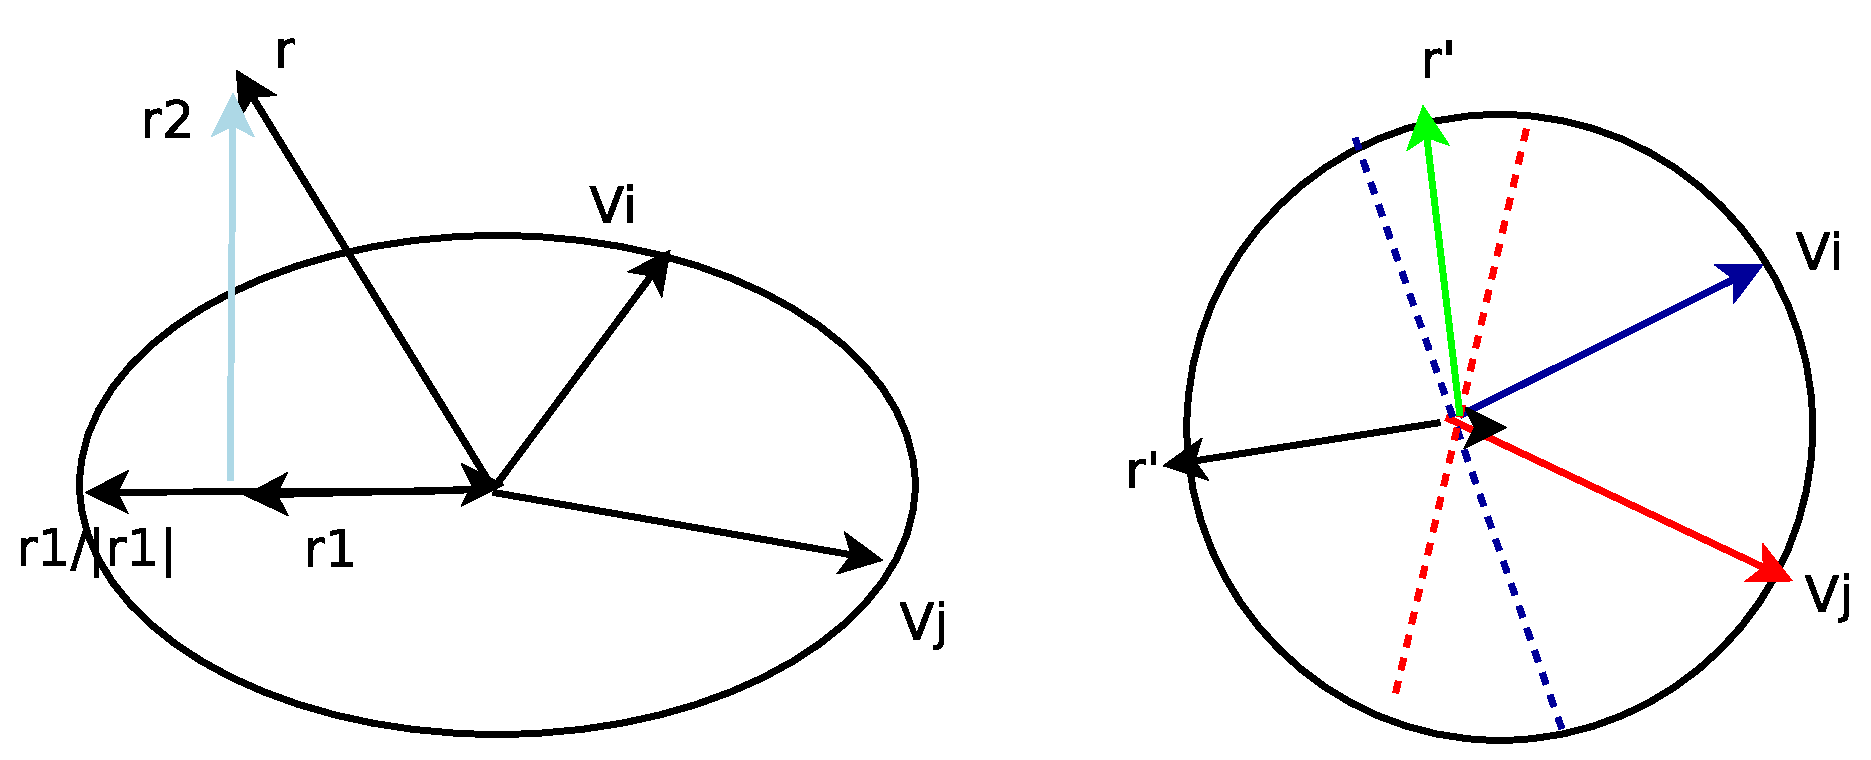
\includegraphics[width=3in]{L20-projection.eps}
\end{figure}


Fact 2: $\Pr[ i \in S \text{ and } j\notin S, \text{ or}   i \notin S \text{ and } j\in S ] = \tfrac{1}{\pi} \arccos( \vec{v_i^*} \bullet \vec{v_j^*} )$. 
(Idea: consider the projection of $\vec{r}$ onto the plane spanned by $\vec{v_i^*}$ and $\vec{v_j^*}$. We have $\vec{v_i^*} \bullet \vec{r} = \vec{v_i^*} \bullet ( \vec{r_1} + \vec{r_2} ) = \vec{v_i^*} \bullet  \vec{r_1} )$ )

Fact 3:  $ \tfrac{1}{\pi} \arccos(x) \geq 0.878 \tfrac{1}{2} (1-x)$ for $-1\leq x \leq 1$. 


\begin{figure}
    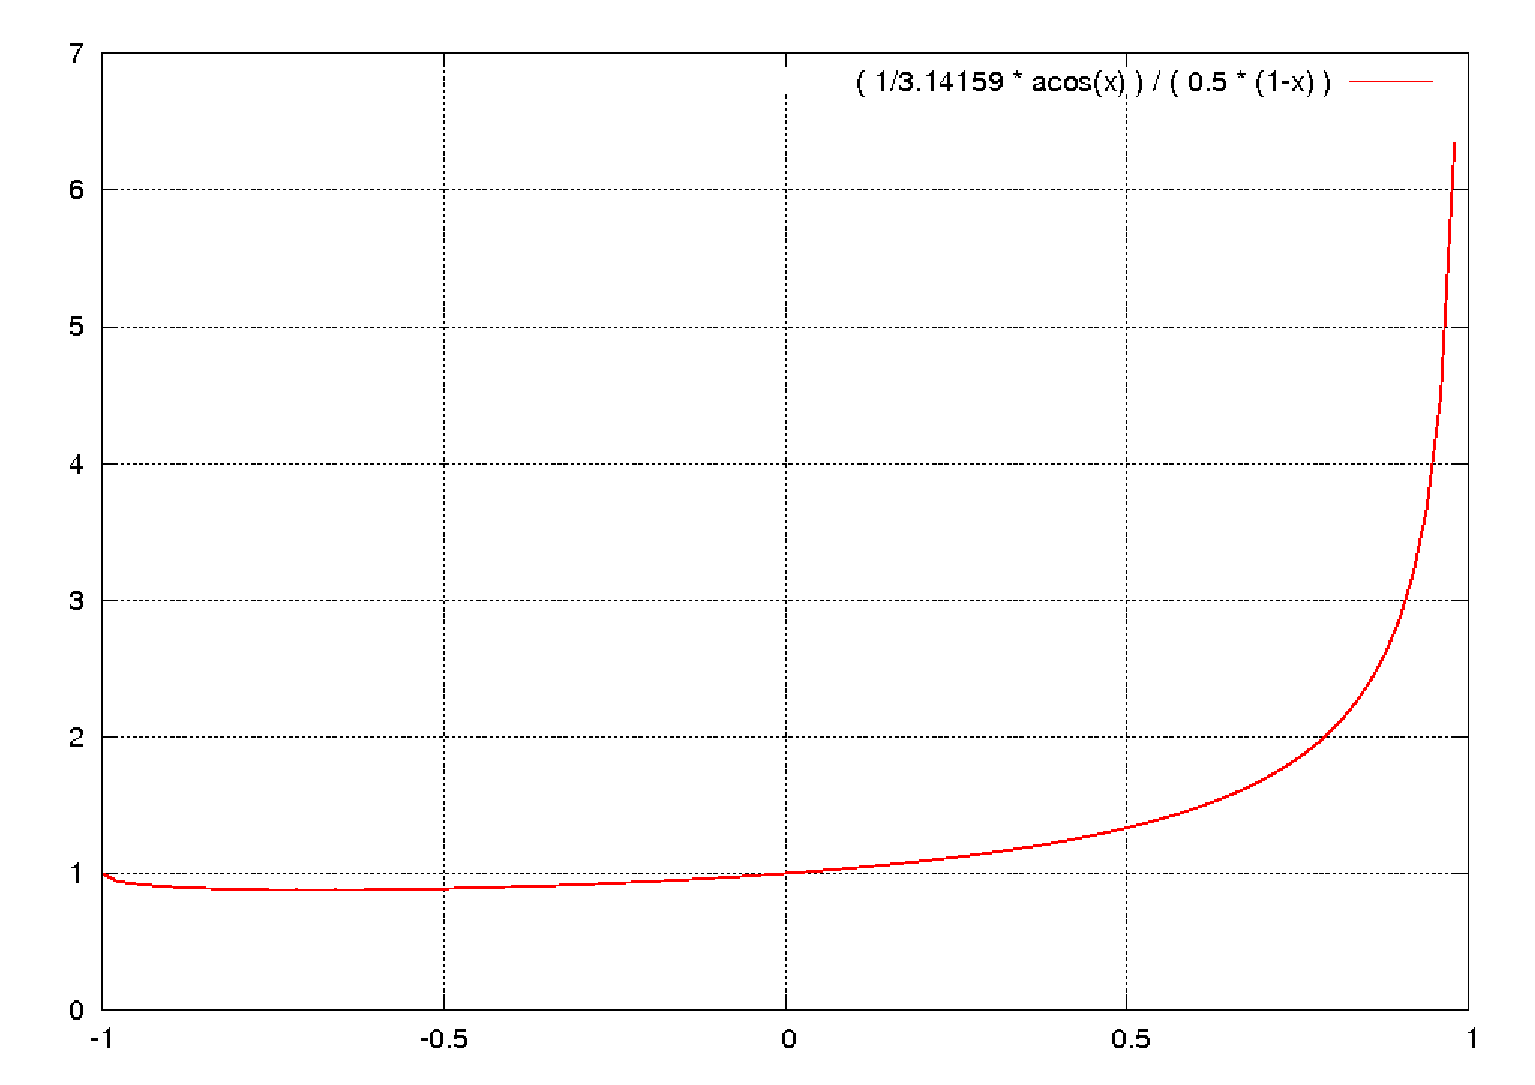
\includegraphics[width=2in]{L20-arccos.eps}
\end{figure}

} 

% \frame{
% \frametitle{Continue}
% 
% $\Pr(x,y|R) = \prod_i q_{x_i} \prod_j q_{y_j}$
%  
%  $\Pr(x,y|M) = \prod_i p_{x_i,y_i}$ 
%  
%  $ \frac{ \Pr(x,y|M) } {\Pr(x,y|R) } = \prod_i \frac{p_{x_i,y_i} }{ q_{x_i} q_{y_i} } $
% 
%  $S=\sum_i s(x_i,y_i)$, where $s(a,b) = \log \frac{p_{ab}}{ q_a q_b }$
%  
%  $\gamma(g) = - d - (g-1) e$
%  
%  $\Pr(gap) = f(g) \prod_{i \text{ in gap} } q_{x_i}$ 
%  
%  $\log( \Pr(gap) ) = \log( f(g) ) + \sum_{ i \text{ in gap} } \log ( q_{x_i} ) $
% 
% }

\end{document}
